%pdflatex -halt-on-error -aux-directory=tmp -output-directory=tmp rapport.tex%

\documentclass{article}
\usepackage{amsmath}
\usepackage[utf8]{inputenc}
\usepackage[T1]{fontenc}
\usepackage{graphicx}
\usepackage{hyperref}
\usepackage[francais]{babel}
\usepackage{listings}
\usepackage{xcolor}

\definecolor{codegreen}{rgb}{0,0.6,0}
\definecolor{codegray}{rgb}{0.5,0.5,0.5}
\definecolor{codepurple}{rgb}{0.58,0,0.82}
\definecolor{backcolour}{rgb}{0.95,0.95,0.92}

\lstdefinestyle{mystyle}{
    language=python,
    backgroundcolor=\color{backcolour},   
    commentstyle=\color{codegreen},
    keywordstyle=\color{magenta},
    numberstyle=\tiny\color{codegray},
    stringstyle=\color{codepurple},
    basicstyle=\ttfamily\footnotesize,
    breakatwhitespace=false,         
    breaklines=true,                 
    captionpos=b,                    
    keepspaces=true,                 
    numbers=left,                    
    numbersep=5pt,                  
    showspaces=false,                
    showstringspaces=false,
    showtabs=false,                  
    tabsize=2
}

\lstset{style=mystyle}

\title{Réseaux II}
\author{Wassim SAIDANE}
\date{Mise à jour du 12/03/2021}

\begin{document}
    \pagenumbering{gobble}
    \maketitle
    \pagenumbering{arabic}
    \tableofcontents
    \newpage
    \section*{Note}
    Ce cours est ma prise de note du cours de L3 info de Raoul Medina.
    \section*{Organisation}
    \section*{\underline{Introduction}}
    \subsection*{Pourquoi étudier les réseaux dans un cours d'informatique ?}  
    -> Les réseaux permettent de partager des ressources. \\
    - Exemple de partage de ressource : Google map. \\ 
    -> \underline{Distribué} vs parallélisme \\
    - Les machines distribuées ont un rapport qualité/prix intéressent.
    Elles permettent une plus grande fiabilité et disponibilité. \\  
    - Les machines distribuées sont également plus extensible. \\
    - Par nature, les applications sont distribuées. \\
    \\
    \subsection*{Un réseau ? C'est quoi ?} 
    C'est un ensemble d'entité interconnecté entre-elles à l'aide de canaux de communications. \\
    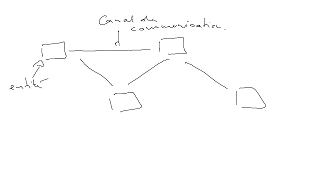
\includegraphics{captures/1.png} \\
    Il existe deux types de canaux : \\ 
    - Point à point (exemple appel téléphonique) : \\
      simplex (unidirectionnel) \\
      full-duplex (biderectionnel et en même temps) \\
      half-duplex. \\
    \newpage
    - Diffusion (Boadcast) \\
    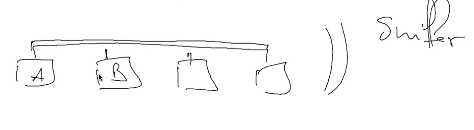
\includegraphics{captures/2.png}
    \subsection*{Quelques caractéristiques des canaux de communication : } 
    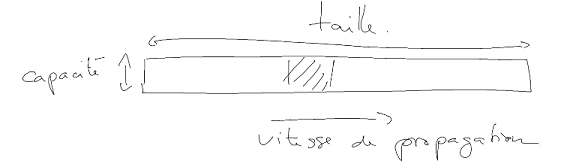
\includegraphics{captures/3.png}
    Quelque soit le canal de communication on aura toujours un taux d'erreurs (une erreur = un bit qui se décale). \\
    vitesse de propagation : $10^{-5}$ bit de parité 50\%\\
    délai de propagation = taille/vitesse de propagation \\
    Temps pour transmettre un bits ? \\
    délai de propagation + $\frac{n}{\text{capacité}} \times \text{taille du paquet en secondes}$ \\
    \\
    \subsection*{Quel est l'objectif du réseau ? } 
    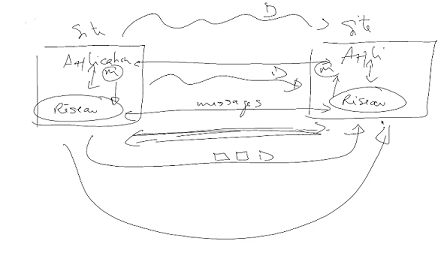
\includegraphics{captures/4.png} \\
    \underline{Problèmes : } \\
    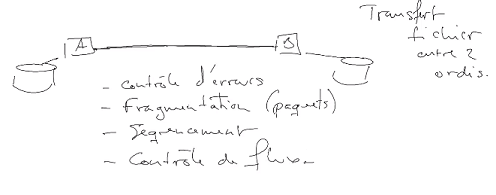
\includegraphics{captures/5.png} \\
    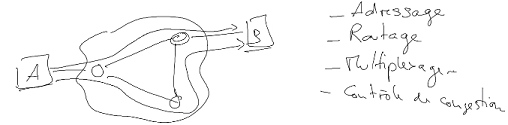
\includegraphics{captures/6.png} \\
    \\
    \newpage
    \section{La couche physique}
    \begin{itemize}
      \item Caractéristique mécaniques
      \item Caractéristique électriques 
      \begin{itemize}
        \item Niveau de volts 
        \item Fréquence de changement de voltage
      \end{itemize}
      \item Caractéristique fonctionelle
      \begin{itemize}
        \item Fonction de chaque broche
      \end{itemize}
      \item Caractéristique procédurale
    \end{itemize}
    Tous ces points définit des standards (Exemple : norme USB). \\
    \underline{Exemples :} \\ 
    \begin{itemize}
      \item Paires torsadées \\
      
\includegraphics{captures/8.PNG} \\
      Exemple : RJ45 \\ 
      \item 50 homes coaxales : 10 base 2, 10 base 5 \\
      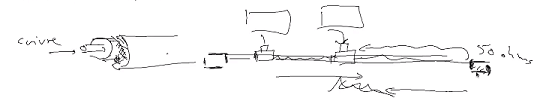
\includegraphics{captures/9.PNG}
      \item 75 homes coaxales -> analogique 
      \item Fibre optique \\
      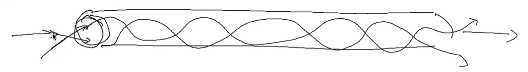
\includegraphics{captures/10.PNG}
      \item Micro-ondes, infrarouge, laser 
      \item Disque externe (clé USB)
    \end{itemize}
    \newpage
    \subsection{Transmission digitale (baseband)}
    Deux niveaux de volttages : \\
    \begin{itemize}
      \item +sv=1
      \item -sv=0
    \end{itemize}
    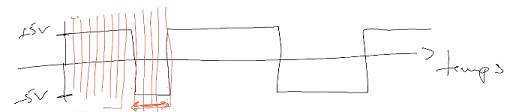
\includegraphics{captures/11.PNG}
    Emetteur et récepteur doivent se mettre d'accord sur la durée d'un bit. \\
    Quelques méthodes : \\ 
    \begin{itemize}
      \item \underline{Cables parallèles} \\
      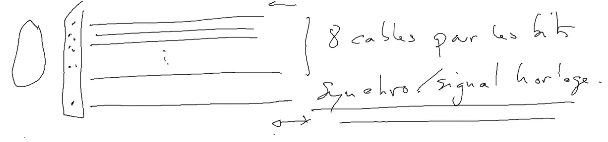
\includegraphics{captures/12.PNG}
      \item \underline{Cables séris}
      \begin{itemize}
        \item Synchrone 
        \item Asynchrone \\
        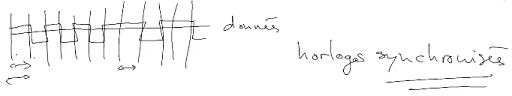
\includegraphics{captures/13.PNG}
      \end{itemize}
    \end{itemize}
    \newpage
    Envoi d'octets : \\ 
    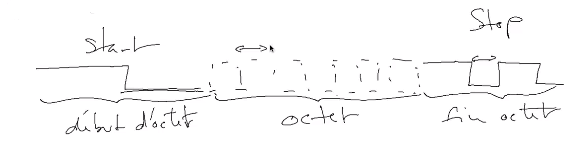
\includegraphics{captures/14.PNG}
    Synchronisation avec chaque bit.
    \\
    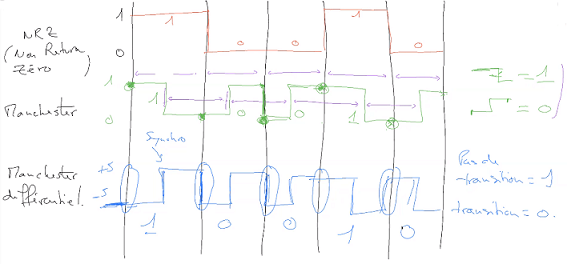
\includegraphics{captures/15.PNG} \\
    Le nombre de changement de signaux par seconde : bonds \\ 
    Soit $x$ le nombre de bonds d'un cnal : \\ 
    bit raté = $\log_2 V \times$ bonds raté \\ 
    v : nombre de signaux \\ 
    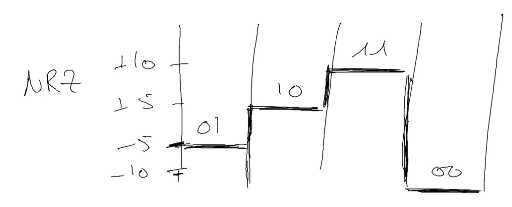
\includegraphics{captures/16.PNG} \\ 
    \underline{Transmission analogique : } \\
    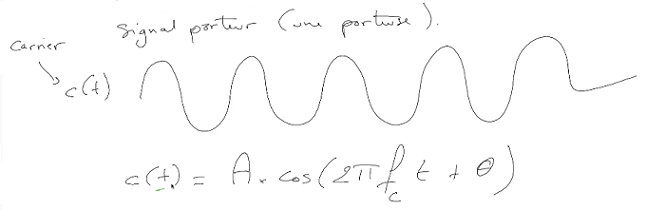
\includegraphics{captures/17.PNG} \\ 
    Transfert se fait par modulation de porteuse : \\ 
    J'ai raté le schéma à cause d'Anthony et Rapha :) \\
    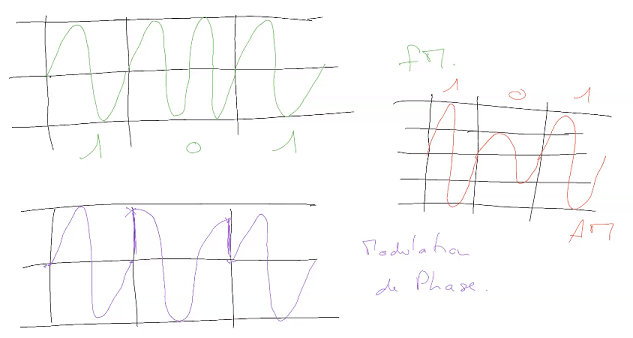
\includegraphics{captures/18.PNG} \\
    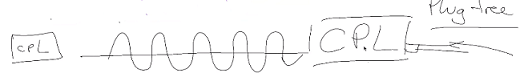
\includegraphics{captures/19.PNG} \\
    Taux de transfert max théorique : \\ 
    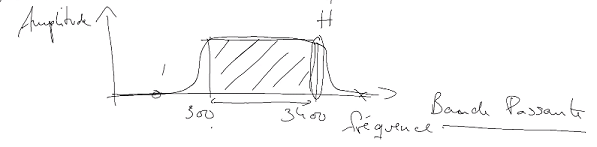
\includegraphics{captures/20.PNG} \\
    Nyquist : TTmax = $2 \times H \times \log_2 V$ \\
    H : Bande passante (fréquence max) \\ 
    V : Nombre de signaux \\
    Shannon : TTmax = $H \times \log_2(1+\frac{S}{B})$ \\ 
    $\frac{S}{B}=$Rapport signal/bruit en décibel. \\ 
    \newpage
    Modemes à haut taux de transferts : \\ 
    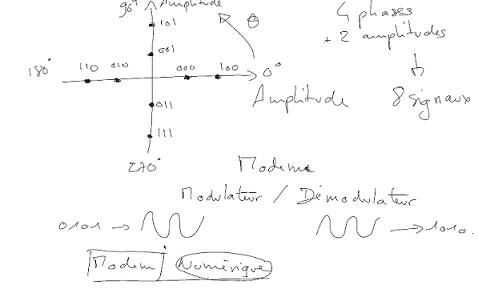
\includegraphics{captures/21.PNG}
\end{document}
